W tym rozdziale przedstawiono przykłady systemów, narzędzi oraz technik nawigacyjnych, które są wykorzystywane w usługach firm komercyjnych 
oraz w dostarczanych przez te firmy systemach rolnictwa precyzyjnego. Z uwagi na niską dostępność specyfikacji technicznych produktów 
dostępnych obecnie na rynku, w pracy ogranioczono się do analizy ofert marketingowych liderów branży maszyn rolniczych.
Jako reprezentatywną próbę dla europejskiego rynku rolnictwa precyzyjnego przyjęto oferty następujących firm: New Holland Agriculture,
John Deere oraz Claas.
\section{Wykorzystanie GNSS}
 test cytowania \cite{CLAAS_stearing_systems}\\
	test cytowania \cite{JOHN_DEERE_solutions}\\
	test cytowania \cite{NEW_HOLLAND_PLM}


\section{Zastosowanie systemów inercjalnych}
Na podstawie analizy ofert marketingowych firm z grupy przyjętej za referencyjną, można wywnioskować, że systemy nawigacji inercjalnej 
są wykorzystywane na potrzeby budowy systemów służących do kompensacji nierówności terenu przy precyzyjnym prowadzeniu maszyn rolniczych.
Firma Trimble w swoich technologiach kompensacji terenu T2, T3 wykorzystuje akcelerometry do wyznaczania kąta inklinacji\footnote{kąt zawarty między osią 
pionową pojazu a kierunkiem siły ciężkości w danym punkcie na Ziemi.} oraz żyroskopy w celu kompensacji danych z akcelerometrów ze względu na własną dynamikę pojazdu oraz 
w celu wyznaczania prędkości z jaką zmienia się położenie pojazdu względem kierunku pionu \cite[]{TRIMBLE}.
Z analizowanej grupy firma John Deere oferuje autorskie rozwiązania w postaci modułu kompensacji terenu TCM. Moduł TCM pozwala na wprowadzanie korekt 
do pozycji GNSS ze względu na pochyłości terenu w trzech osiach z, y, z. Moduł kompensacji terenu jest domyślenie zintergrowany z odbiornikiem GNSS StarFire 3000.
Rysunek \ref{fig:john_deere_tcm} przedstawia możliwości systemu TCM. 

\begin{figure}[H]
\centering
\begin{minipage}[c]{0.6\linewidth}
  \begin{flushleft}
  	\begin{minipage}[t]{0.5\linewidth}
		\raggedleft
		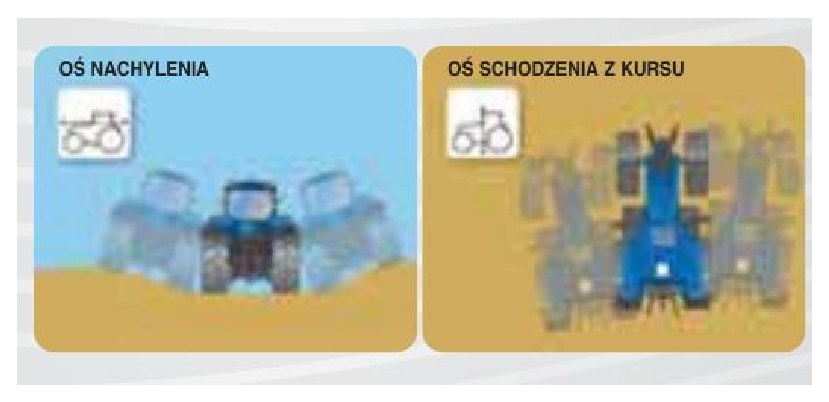
\includegraphics[scale = 0.4]{ch5_new_holland_terrain_compensation_t2.eps}	
		\label{fig:t2}
		\subcaption{Technologia kompensacji terenu T2 wykorzystywana przez New Holland Agriculture}
	\end{minipage}
	\vfill
	\begin{minipage}[b]{0.5\linewidth}
		\raggedleft
		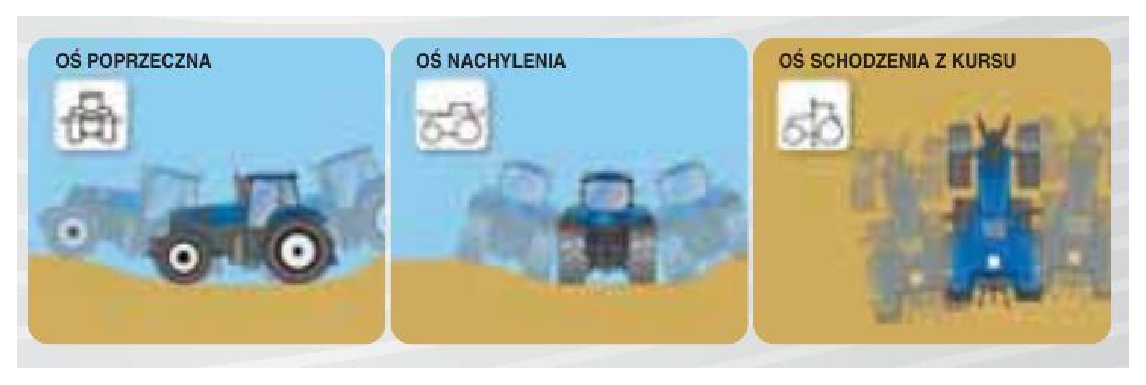
\includegraphics[scale = 0.4]{ch5_new_holland_terrain_compensation_t3.eps}
		\label{fig:t3}
		\subcaption{Technolohia kompenasacji terenu T3 wykorzystywana przez New Holland Agriculture}
	\end{minipage}
  \end{flushleft}
\end{minipage}%
\hfill
\begin{minipage}[c]{0.4\linewidth}
  \begin{flushright}
  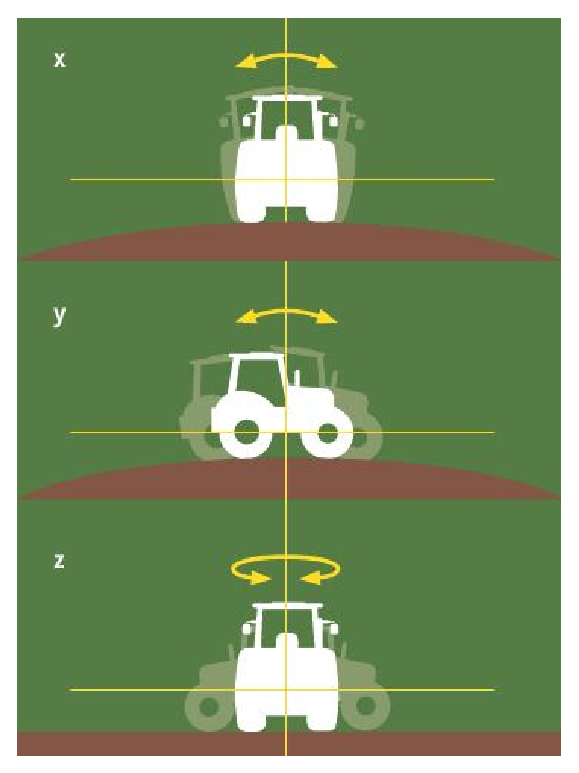
\includegraphics[scale = 0.5]{ch5_john_deere_terrain_compensation.eps}
  \label{fig:john_deere_tcm}
  \subcaption{\textit{Technologia kompensacji terenu TCM od John Deere} źródło \cite[][strona 8]{JOHN_DEERE_solutions}}
  \end{flushright}
\end{minipage}
\caption{\textit{Kompensacja wpływu nierówności terenu na pozycję GNSS}}
\label{fig:terrain_compensation}
\end{figure}
Firma New Holland Agriculture również posiada w swojej ofercie system kompensacji terenu w dwóch różnych wersjach: T2 - z pominięciem kompensacji w 
płaszczyźnie podłużnej, T3 - kompensujący nierówności w obu płasczyznach (poprzeczna, podłużna) oraz zapobiegający schodzeniu maszyny z kursu \cite[][strona 7]{NEW_HOLLAND_PLM}.
Firma New Holland Agriculture najprawdopodobniej wykorzystuje rozwiązania T2 oraz T3 oferowane przez odbiorniki marki Trimble. 
Na rysunku \ref{fig:t2} oraz \ref{fig:t3} przedstawiono schemat działania rozwiązań zaadoptowanych przez New Holland.
Z reprezentatywnej grupy firm tylko Class nie przedstawił w swojej broszurze oferty korekt GNSS ze względu na nierówności terenu.\\
\indent Warto nadmienić, że firmy obecnie jedynie wykorzystują narzędzia nawigacji inercjalnej (INS) do korekcji rozwiązań GNSS.
Z broszur marketingowych wywnioskować można, że komercyjnie nie stosuje się jeszcze filtru kalmana w celu wspólnego opracowania obserwacji GNSS plus INS.
\section{Zastosowanie sensorów video}
Firma CLASS w swojej ofercie posiada systemy wspomagające nawigację GNSS oparte o sensory wideo. CAM PILOT przedstawiony na rysunku \ref{fig:class_cam_pilot1}
jest systemem automatycznego kierowania sterowanym przez kamerę stereoskopową. Został zaprojektowany specjalnie do zbioru traw. Kamera ustala pozycję pokosów 
i na podstawie tej informacji odbywa się prowadzenie pojazdu \cite[][strona 7]{CLAAS_stearing_systems}.
W ofercie firmy CLASS jest także system oparty na skaningu laserowym LASER PILOT zobrazowany na 
rysunku \ref{fig:class_laser_pilot1} zaprojektowany do ustalania krawędzi między polem skoszonym a jeszcze nie omłuconym. System pozwala na 
prowadzenie pojazdu wzdłuż tej krawędzi z dokładnością 10-20cm \cite[][strona 6]{CLAAS_stearing_systems}.
\begin{figure}[H]
\centering
	\begin{subfigure}{0.4\textwidth}
		\centering
		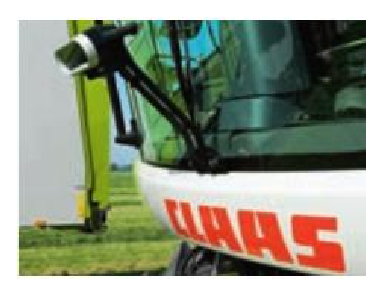
\includegraphics[width=0.9\linewidth]{ch5_class_cam_pilot0.eps}
		\label{fig:class_cam_pilot1}
		\caption{CLASS CAM PILOT}
	\end{subfigure}
	%\hfill
	\begin{subfigure}{0.4\textwidth}
                \centering
                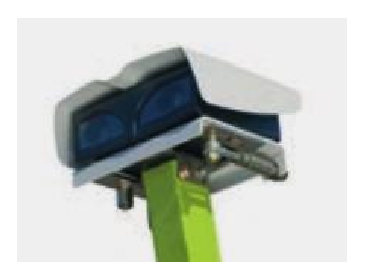
\includegraphics[width=0.9\linewidth]{ch5_class_laser_pilot0.eps}
                \label{fig:class_laser_pilot1}
                \caption{CLASS LASER PILOT}
	\end{subfigure} \\
	\vfill
	\begin{subfigure}{0.4\textwidth}
                \centering
                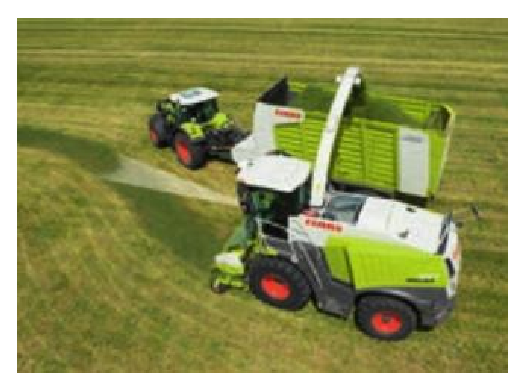
\includegraphics[width=0.9\linewidth]{ch5_class_cam_pilot.eps}
                \label{fig:class_cam_pilot2}
                \caption{CLASS CAM PILOT podczas pracy}
	\end{subfigure}
	\begin{subfigure}{0.4\textwidth}
                \centering
                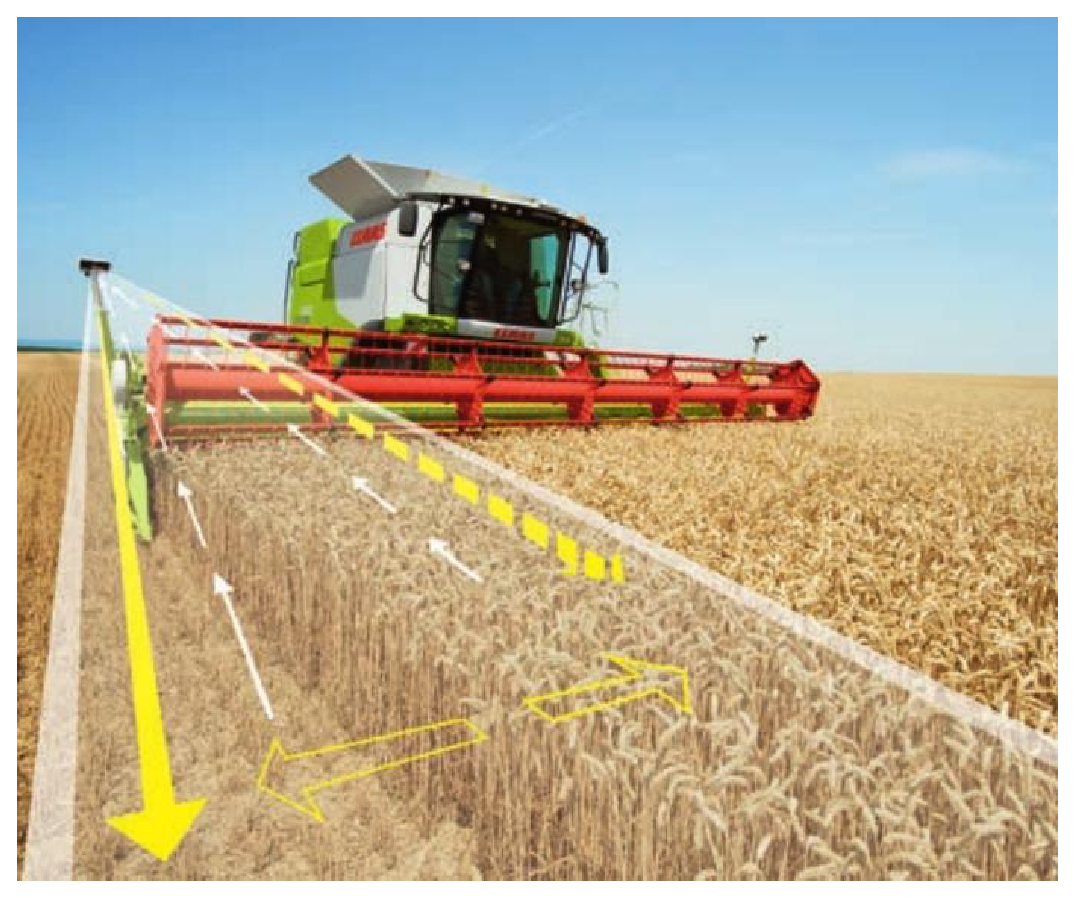
\includegraphics[width=0.9\linewidth]{ch5_class_laser_pilot.eps}
                \label{fig:class_laser_pilot2}
                \caption{CLASS LASER PILOT podczas pracy}
	\end{subfigure}
\caption{Systemy bazujące na sensorach wideo marki CLASS}
\end{figure}
\indent Również firma New Holland Agriculture posiada w swej ofercie system oparty na sensorach wideo.
System SMARTSTEER przedstawiony na rysunku \ref{fig:new_holland_smartsteer} za pomocą skanera laserowego wytycza krawędź dzielącą ściernisko 
od zborza i na podstawie tej informacji przesyła sygnały do układu kierowniczego \cite[][strona 18]{NEW_HOLLAND_PLM}.
\begin{figure}[H]
	\centering
	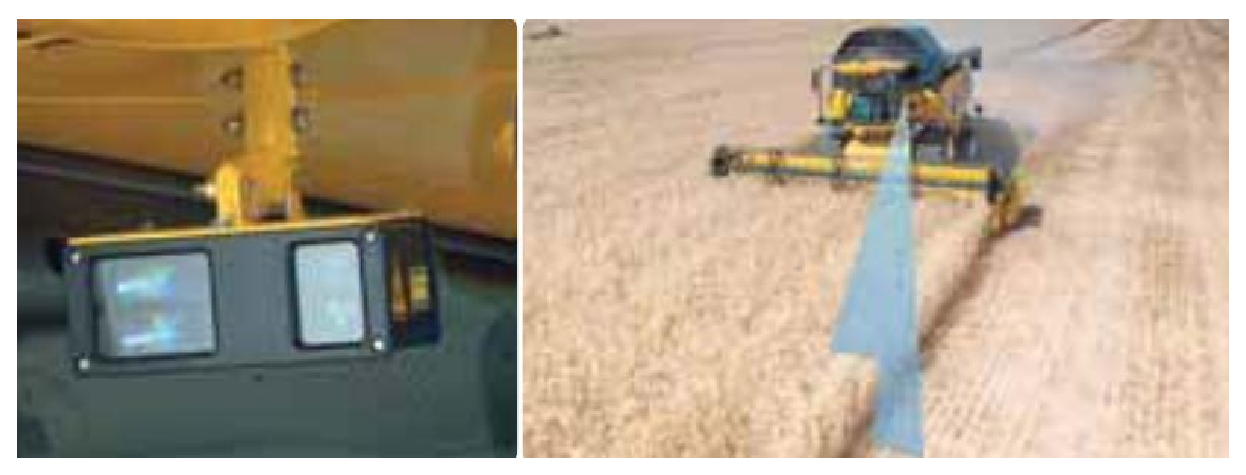
\includegraphics[width=0.7\linewidth]{ch5_new_holland_laser_pilot.eps}
	\caption{System SMARTSTEER firmy New Holland Agriculture}
	\label{new_holland_smartsteer}
\end{figure}
\indent Firma John Deere jako jedyna firma z trzech wybranych do analizy, nie prezentuje rozwiązań opartych o czujniki optyczne w swojej ofercie dotyczącej 
systemów prowadzenia.
\indent Podobnie jak w przypadku danych z sensorów INS, tak i dane pochodzące z sensorów wideo nie są jeszcze przetwarzane komercyjnie
za pomocą algorytmów fuzji danych łącznie z danymi nawigacyjnymi GNSS.  
\indent Na zakończenie tego podrozdziału warto krytycznie spojrzeć na dokładności systemów optycznych w zastosowanich do zbioru plonów.
Jeżeli nawet prawdą jest uzyskanie dokładności 10cm, to na odcinku o długości 100m statystycznie pozostawimy nieomłócony obszar równy 5$m^2$.
Przy załorzeniu szerokości hedera 10m otrzymujemy błąd na poziomie pięciu promili, co daje maksymalnie 40kg na hektar. 
W przypadku pesymistycznym, zakładając błąd prowadzenia rzędu 30cm stracimy około kwintala zborza. 
W realiach polskigo rolnictwa, przy dużym rozdrobnieniu urzytków rolnych lepiej jest stracić nawet dwa kwintale zborza lub 
dać zarobić ten ekwiwalent operatorowi kombajnu niż inwestować w drogie systemy prowadzenia.

